
% Inbuilt themes in beamer
\documentclass[aspectratio=169]{beamer}
\usepackage{graphicx}
\usepackage{amsmath}
% Theme choice:
\usetheme{CambridgeUS}

% Title page details: 
\title{Chapter 15: Monopoly} 
\author{Discussion section 4}
\date{Apr 2024}

\begin{document}

% Title page
\begin{frame}
    \titlepage 
\end{frame}

\begin{frame}{Monopolies}
    \begin{center}
        Is Amazon a monopoly?
    \end{center}
\end{frame}

\begin{frame}{Monopolies}
        \begin{center}
            What are some monopolies you encounter?
        \end{center}
\end{frame}

\begin{frame}{Monopolies}
    \begin{center}
        What are some monopolies you encounter?
    \end{center}
    \begin{itemize}
        \item BG\&E
        \item Verizon (certain neighborhoods)
        \item Post office
    \end{itemize}
\end{frame}

% Outline frame
\begin{frame}{Outline}
    \begin{itemize}
        \item We have focused so far on \textit{competitive firms}; now we will look at monopolies
        \item This means firms with \textit{market power}
        \begin{itemize}
            \item Instead of price \textit{takers} they are price \textit{makers}
        \end{itemize}
        \item Look at their behavior, implications for welfare, and government responses
    \end{itemize}

    \vspace{5mm}

    But first: what \textit{is} a monopoly?
\end{frame}

\begin{frame}{Characteristics of monopolies}
    Monopolies:
    \begin{itemize}
        \item Produce goods with no close substitutes
        \item Are the sole provider of that good
        \item Can set prices as a result of 1 and 2
    \end{itemize}

    \vspace{5mm}

    Why might a monopoly emerge?
\end{frame}

\begin{frame}{Reasons for monopolies}
    Why might a monopoly emerge?

    \vspace{2mm}

    \begin{itemize}
        \item Resources (mine for a rare resource)
        \item Regulations (patents and copyright)
        \item Production process (natural monopolies, economies of scale, network effects)
    \end{itemize}

    If monopolies can set prices, how will they decide how much to produce/at what price?
\end{frame}

\begin{frame}{Pricing decision}
    \begin{itemize}
        \item How does a monopoly decide on its production?
        \item Just like the firm in the competitive market, monopolies want to maximize profits
        \item Set price too high, no one will buy the good; find the ``sweet spot''
    \end{itemize}

    \vspace{2mm}

    What is the demand curve that a monopoly faces? Why?
\end{frame}

\begin{frame}{Demand curve}
    \begin{itemize}
         \item In a competitive market, no matter what quantity a firm produces, they sell at the market price; a \textit{vertical demand curve}
         \item With a monopoly, the demand curve is now \textit{downward sloping}
        \item Now, the firm \textit{sets the market price} by their output decision
    \end{itemize}

    \vspace{5mm}

    Thus we return to the demand curve from the free market equilibrium.

    \vspace{2mm}

    What happens to total revenue if we increase quantity?
\end{frame}

\begin{frame}{Demand}
    What happens to total revenue if we increase quantity?
    
    \begin{itemize}
        \item Remember, TR = Q * P
        \item So there will be two effects:
        \begin{itemize}
            \item Output (direct) effect: increase Q $\to$ higher revenue
            \item Price (indirect) effect: increase Q $\to$ decreased P $\to$ lower revenue
            \item (Note: for competitive firm, price effect is 0)
        \end{itemize}
        \item Not clear ex ante which will dominate!
    \end{itemize}
\end{frame}

\begin{frame}{Demand curve}
    \centering
    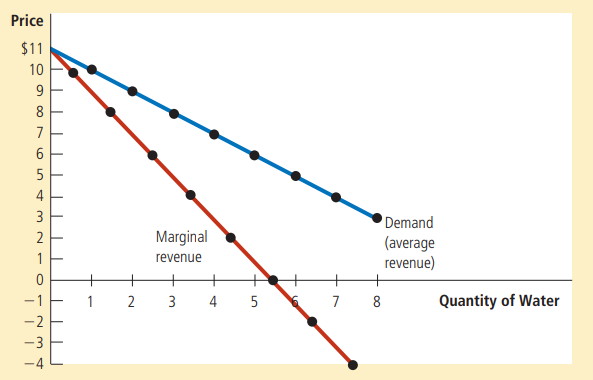
\includegraphics[width = 0.6\textwidth,keepaspectratio]{demandMR.png}
\end{frame}

\begin{frame}{Profit maximization}
    Note that P  = AR.
        
    \vspace{5mm}

    Where does the profit maximizing firm want to produce? 
\end{frame}

\begin{frame}{Profit maximization}
    Where does the profit maximizing firm want to produce? 

    \begin{itemize}
        \item Still where MR = MC!
        \item If they produce below, there is extra profit to be made
        \item If they produce above, they are losing profits on additional units
    \end{itemize}
\end{frame}

\begin{frame}{Profit maximization}
    \centering
    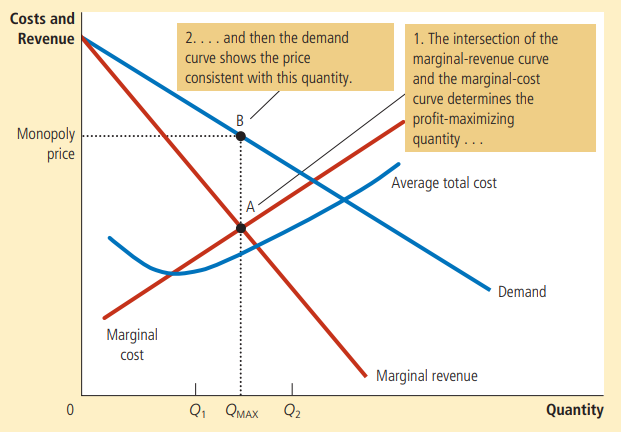
\includegraphics[width = 0.6\textwidth,keepaspectratio]{profitmax.png}
\end{frame}

\begin{frame}{Profit maximization}
    \begin{itemize}
        \item For the competitive firm, P = MC = MR
        \item For the monopolist, P $>$ MC = MR
        \item Producing at a lower quantity!
    \end{itemize}

    \begin{equation*}
        \begin{split}
            \Pi & = TR - TC \\
            \Pi & = (TR/Q - TC/Q)*Q \\
            \Pi & = (P - ATC) * Q
        \end{split}
    \end{equation*}
\end{frame}

\begin{frame}{Profit maximization}
    \centering
    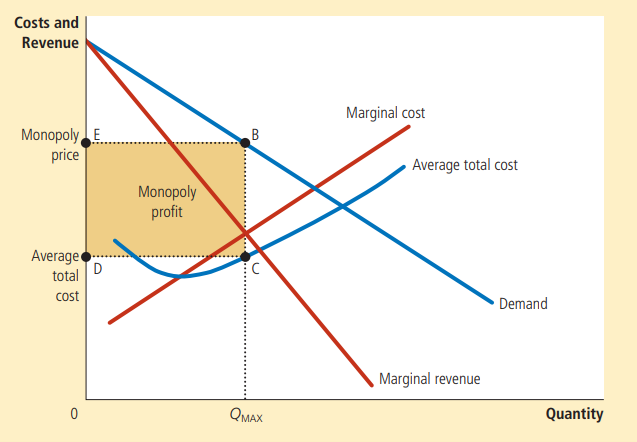
\includegraphics[width = 0.6\textwidth,keepaspectratio]{totalprofit.png}
\end{frame}

\begin{frame}{Welfare}
    So, what does all this mean for society?

    \vspace{2mm}

    Is it good or bad? 

    \vspace{2mm}

    How do we know?
\end{frame}

\begin{frame}{Welfare}
    For a normative evaluation, we need to return to our tools of \textit{welfare economics}.

    \begin{itemize}
        \item Consumers pay more than they otherwise would have, and fewer are able to enjoy the good because of lower quantity
        \begin{itemize}
            \item This suggests CS is decreasing
        \end{itemize}
        \item But, the firm receives more revenue! So they are happy.
        \item What happens to total surplus? Is there any DL?
    \end{itemize}
\end{frame}

\begin{frame}{Profit maximization}
    \centering
    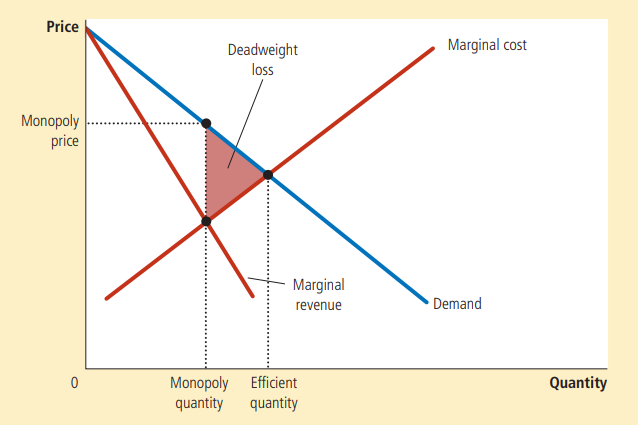
\includegraphics[width = 0.6\textwidth,keepaspectratio]{
     DL.png}
\end{frame}

\begin{frame}{Welfare}
    \begin{itemize}
        \item DL similar to presence of a tax
        \item In fact, monopoly operates much like the government
        \item Or --- government operates like a monopoly?
        \item Intuitively, DL comes from lower supply
    \end{itemize}
\end{frame}

\begin{frame}{Price discrimination}
    We have assumed all consumers face the same price.

    \vspace{2mm}

    Could they charge different prices to different types of consumers? Why?
\end{frame}

\begin{frame}{Price discrimination}
    This is called \textit{price discrimination}.

    \begin{itemize}
        \item Requires market power
        \item May be perfectly rational
        \item Requires ability to distinguish between buyers
        \item Might be welfare improving!
        \begin{itemize}
            \item How could this possibly be true??
        \end{itemize}
    \end{itemize}
\end{frame}

\begin{frame}{Welfare}
    \centering
    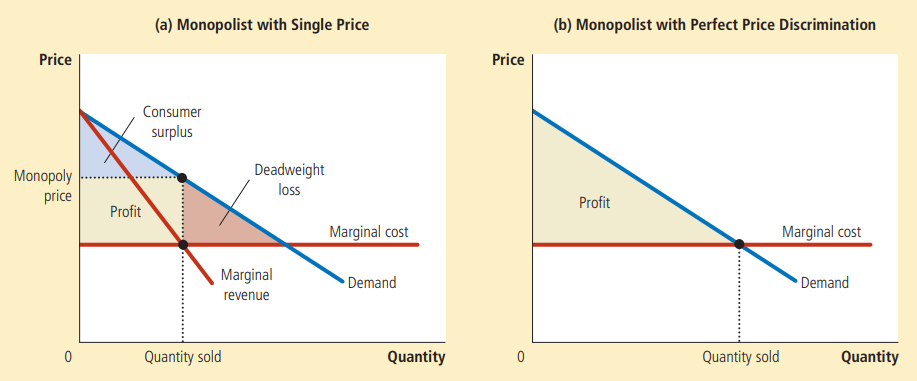
\includegraphics[width = 0.8\textwidth,keepaspectratio]{pricediscrim.png}
\end{frame}

\begin{frame}{Government}
    OK, so presence of a monopoly might lead to welfare loss.

    \vspace{2mm}

    What might the government do to try and improve welfare?
\end{frame}

\begin{frame}{Government}
    OK, so presence of a monopoly might lead to welfare loss.

    \vspace{2mm}

    What might the government do to try and improve welfare?

    \vspace{5mm}

    \begin{itemize}
        \item Antitrust (breaking up AT\&T)
        \item Regulation: cap or subsidize prices
        \item Public ownership
    \end{itemize}
\end{frame}

\end{document}
